\documentclass[onepage]{beamer}
\mode<presentation>{
	\setbeamercovered{transparent}
	%\beamertemplatenavigationsymbolsempty
	\setbeamertemplate{footline}[frame number]
% 	\usefonttheme{professionalfonts}
}

% https://tex.stackexchange.com/questions/34166/understanding-minipages-aligning-at-top
\usepackage{adjustbox}

% https://tex.stackexchange.com/questions/124256/how-do-i-get-numbered-entries-in-a-beamer-bibliography
\setbeamertemplate{bibliography item}{\insertbiblabel}

% https://tex.stackexchange.com/questions/49048/how-to-cite-one-bibentry-in-full-length-in-the-body-text
\usepackage{bibentry}
\bibliographystyle{plain}
\nobibliography*
%
% https://tex.stackexchange.com/questions/163827/wrong-vertical-spaces-using-bibentry-within-beamer/163842
\def\mybeamernewblock{%
  \usebeamercolor[fg]{bibliography entry author}%
  \usebeamerfont{bibliography entry author}%
  \usebeamertemplate{bibliography entry author}%
  \def\newblock{%
    \usebeamercolor[fg]{bibliography entry title}%
    \usebeamerfont{bibliography entry title}%
    \usebeamertemplate{bibliography entry title}%
    \def\newblock{%
      \usebeamercolor[fg]{bibliography entry location}%
      \usebeamerfont{bibliography entry location}%
      \usebeamertemplate{bibliography entry location}%
      \def\newblock{%
        \usebeamercolor[fg]{bibliography entry note}%
        \usebeamerfont{bibliography entry note}%
        \usebeamertemplate{bibliography entry note}}}}%
  \leavevmode
}
\newenvironment{references}{\begin{itemize}\let\newblock\mybeamernewblock}{\end{itemize}}


\setbeamersize{text margin left=10pt, text margin right=10pt}
\setbeamertemplate{itemize items}[circle]

\beamertemplatenavigationsymbolsempty

% http://tex.stackexchange.com/questions/8680/how-can-i-insert-a-newline-in-a-framebox
%\usepackage{minibox}
%\usepackage{framed}
%\usepackage[usestackEOL]{stackengine}

% % http://tex.stackexchange.com/questions/167000/annotating-tables-with-tikz-adding-arrows
% \usepackage{color, colortbl}
\usepackage{tikz}
\tikzstyle{every picture}+=[remember picture]
%\usetikzlibrary{tikzmark, positioning, fit, shapes.misc}

%% http://tex.stackexchange.com/questions/91124/itemize-removing-natural-indent
%\usepackage{enumitem}

%% http://tex.stackexchange.com/questions/41408/a-five-level-deep-list
%\usepackage{enumitem}
%\setlistdepth{9}

% https://tex.stackexchange.com/questions/20792/how-to-superimpose-latex-on-a-picture
\usepackage{overpic}

% % http://tex.stackexchange.com/questions/32661/how-to-locate-figures-with-x-y-specified-location-in-a-presentation
% \usepackage[absolute,overlay]{textpos} % absolute positioning of stuff
% \setlength{\TPHorizModule}{1mm}
% \setlength{\TPVertModule}{1mm}

\usepackage{graphicx}
\graphicspath{{../img/}}
\AtBeginDocument{\DeclareGraphicsExtensions{.eps, .png, .gif, .pdf}}

\usepackage[makeroom]{cancel}

\usepackage[english]{babel}
\usepackage[T1]{fontenc}
\usepackage{times}

% \usepackage{amssymb}
% \usepackage{nicefrac}
% \usepackage{bbm}
% \usepackage{esint}
% \usepackage{sidecap}

\usepackage{hyperref}
% \hypersetup{pdfpagemode=FullScreen}

\newcommand{\HIDE}[1]{}

\newcommand{\skipline}{{\ }\\}

\newcommand{\EMAIL}{{\color{blue}randreev{\tiny\color{white}.\hspace{-1.5pt}}@{\tiny\color{white}.\hspace{-1.5pt}}stat.sinica.edu.tw}}

\author{\small RA}
\subject{Talks}

\newcommand{\CITE}[1]{{\footnotesize[#1]}}

% \input{definitions}

\providecommand{\DIV}{\mathop{\text{div}}}
\providecommand{\GRAD}{\mathop{\text{grad}}}

\providecommand{\IE}{\mathbb{E}}
\providecommand{\IP}{\mathbb{P}}
\providecommand{\IR}{\mathbb{R}}
\providecommand{\IZ}{\mathbb{Z}}

\providecommand{\duality}[2]{\langle #1 \rangle_{#2}}
\providecommand{\norm}[2]{\| #1 \|_{#2}}
\providecommand{\seminorm}[2]{| #1 |_{#2}}
\providecommand{\VERT}{\ensuremath{| \! | \! |}}
\newcommand{\tnorm}[2]{\VERT{#1}\VERT_{{#2}}}

\newcommand{\cA}{\mathcal{A}}
\newcommand{\cB}{\mathcal{B}}
\newcommand{\cL}{\mathcal{L}}
\newcommand{\cN}{\mathcal{N}}
\newcommand{\cT}{\mathcal{T}}
\newcommand{\cX}{\mathcal{X}}
\newcommand{\cY}{\mathcal{Y}}

\providecommand{\Abf}{\mathbf{A}}
\providecommand{\Bbf}{\mathbf{B}}
\providecommand{\Dbf}{\mathbf{D}}
\providecommand{\Ibf}{\mathbf{I}}
\providecommand{\Jbf}{\mathbf{J}}
\providecommand{\Fbf}{\mathbf{F}}
\providecommand{\Hbf}{\mathbf{H}}
\providecommand{\Mbf}{\mathbf{M}}
\providecommand{\Tbf}{\mathbf{T}}
\providecommand{\Pbf}{\mathbf{P}}
\providecommand{\Vbf}{\mathbf{V}}
\providecommand{\pbf}{\mathbf{p}}
\providecommand{\ubf}{\mathbf{u}}
\providecommand{\vbf}{\mathbf{v}}
\providecommand{\wbf}{\mathbf{w}}
\providecommand{\ybf}{\mathbf{y}}
\providecommand{\zbf}{\mathbf{z}}

\renewcommand{\vec}[1]{\mathbf{#1}}

\providecommand{\T}{\mathsf{T}}

\renewcommand{\hat}[1]{\widehat{#1}}
\renewcommand{\tilde}[1]{\widetilde{#1}}

\newcommand{\rd}{\,\mathrm{d}}

\newcommand{\TEXT}[1]{\quad\text{#1}\quad}

% http://tex.stackexchange.com/questions/211518/beamer-vfill-and-itemize
\def\Bottom#1{\vskip 0pt plus 1filll #1}
\def\BottomRight#1{\Bottom{\hfill #1}}

% MATLAB CODE LISTING
\usepackage{color}
\definecolor{DarkBlue}{rgb}{0,0,0.4}
% \definecolor{DarkRed}{rgb}{0.3,0,0}
\definecolor{DarkGreen}{rgb}{0,0.3,0}
\usepackage{listings}
\lstset{%
	language=MATLAB,
	basicstyle=\bf\ttfamily\tiny,%\footnotesize,
	keywordstyle=\color{DarkBlue},
	numbers=left, numberstyle=\footnotesize, numbersep=4pt,
	commentstyle={\color{DarkGreen}},
% 	backgroundcolor=\color{white},
	showspaces=false, showstringspaces=false, showtabs=false,
	frame=none,
	tabsize=4,
	breaklines=true, breakatwhitespace=false,
	emph={[1]femT_,femT_assemE,femT_assemF,femT_assemFE,femTX_assemLoad,spacetime},
	emphstyle={[1]\color{blue}},
	emph={[2]femX_,femX_MA,femX_b,femX_init,femX_show},
	emphstyle={[2]\color{DarkGreen}},
	morekeywords={parfor,true,false},
	xleftmargin=8pt,
	numbers=none
}


%%%%%%%%%%%%%%%%%%%%%%%%%%%%%%%%%%%%%%%%%%%%%%%%%%%%%%%%%%%%%%%%%%%%%%%%%%%%%%%%
%%
%%%%%%%%%%%%%%%%%%%%%%%%%%%%%%%%%%%%%%%%%%%%%%%%%%%%%%%%%%%%%%%%%%%%%%%%%%%%%%%%

\usepackage{ifthen}

\newcommand{\REDBOX}[1]{
	\setlength{\fboxrule}{1pt}
	\fcolorbox{red}{SeeMeBarely}{$\displaystyle
		#1
	$}
}

\definecolor{SeeMeBarely}{RGB}{230,230,230}
\definecolor{Purple}{RGB}{128,0,128}
\definecolor{DeepPurple}{RGB}{32,0,96}
\newcommand{\ra}[1]{{\color{blue}{#1}}}
\newcommand{\cred}[1]{{\color{red}{#1}}}
\newcommand{\cblu}[1]{{\color{blue}{#1}}}
\newcommand{\cpur}[1]{{\color{Purple}{#1}}}

\DeclareMathOperator*{\argmin}{arg\,min}

\newcommand{\ItemComment}[1]{\hfill{\scriptsize(#1)\normalsize}}


% http://www.webnots.com/vibgyor-rainbow-color-codes/
\definecolor{a}{RGB}{148, 0, 211}
\definecolor{b}{RGB}{75, 0, 130}
\definecolor{c}{RGB}{0, 0, 255}
\definecolor{d}{RGB}{0, 160, 0}
\definecolor{e}{RGB}{200, 200, 0}
\definecolor{f}{RGB}{255, 127, 0}
\definecolor{g}{RGB}{255, 0, 0}
%
\definecolor{z}{RGB}{0, 0, 0}
\definecolor{w}{RGB}{255, 255, 255}

% http://tex.stackexchange.com/questions/17611/how-does-one-type-chinese-in-latex
\usepackage{CJKutf8}
\AtBeginDvi{\input{zhwinfonts}}
%
\newcommand{\REN}{\begin{CJK*}{UTF8}{gbsn}人\end{CJK*}}
\newcommand{\ren}[1]{{\color{#1}\REN}}



%%%%%%%%%%%%%%%%%%%%%%%%%%%%%%%%%%%%%%%%%%%%%%%%%%%%%%%%%%%%%%%%%%%%%%%%%%%%%%%%
\begin{document}
%%%%%%%%%%%%%%%%%%%%%%%%%%%%%%%%%%%%%%%%%%%%%%%%%%%%%%%%%%%%%%%%%%%%%%%%%%%%%%%%
%%%%%%%%%%%%%%%%%%%%%%%%%%%%%%%%%%%%%%%%%%%%%%%%%%%%%%%%%%%%%%%%%%%%%%%%%%%%%%%%

%%%%%%%%%%%%%%%%%%%%%%%%%%%%%%%%%%%%%%%%%%%%%%%%%%%%%%%%%%%%%%%%%%%%%%%%%%%%%%%%
\section{Intro}
%%%%%%%%%%%%%%%%%%%%%%%%%%%%%%%%%%%%%%%%%%%%%%%%%%%%%%%%%%%%%%%%%%%%%%%%%%%%%%%%



\begin{frame}[plain,t]
	\begin{center}
		%\small
		%
		Some stats on the GSE75688 BC dataset
		%
		\\[1\baselineskip]
		\small
		RA
% 		\\[1\baselineskip]
% 		\footnotesize
% 		ISS, AS \\ \EMAIL

		\vspace{1cm}

		%

	\end{center}

	\Bottom{
		\scriptsize
		%Support: 
		\hfill
		Dec, 2017
		\\ {\ }
	}
\end{frame}

%%%

\begin{frame}[t]{Silhouette plots}{}
	\begin{center}
		\begin{overpic}[width=0.8\textwidth]{1_plots/silhouette_z=False}
			\put(0, 0) {\scriptsize Original data, Euclidian distance}
		\end{overpic}
		
		{\ }
		
		\begin{overpic}[width=0.8\textwidth]{1_plots/silhouette_z=True}
			\put(0, 0) {\scriptsize Gene-wise Z transform, Euclidian distance}
		\end{overpic}
	\end{center}
\end{frame}

%%%

\begin{frame}[t]{Differential expression (KS distance max/tumors)}{Hand-picked GO terms}
	\begin{center}
		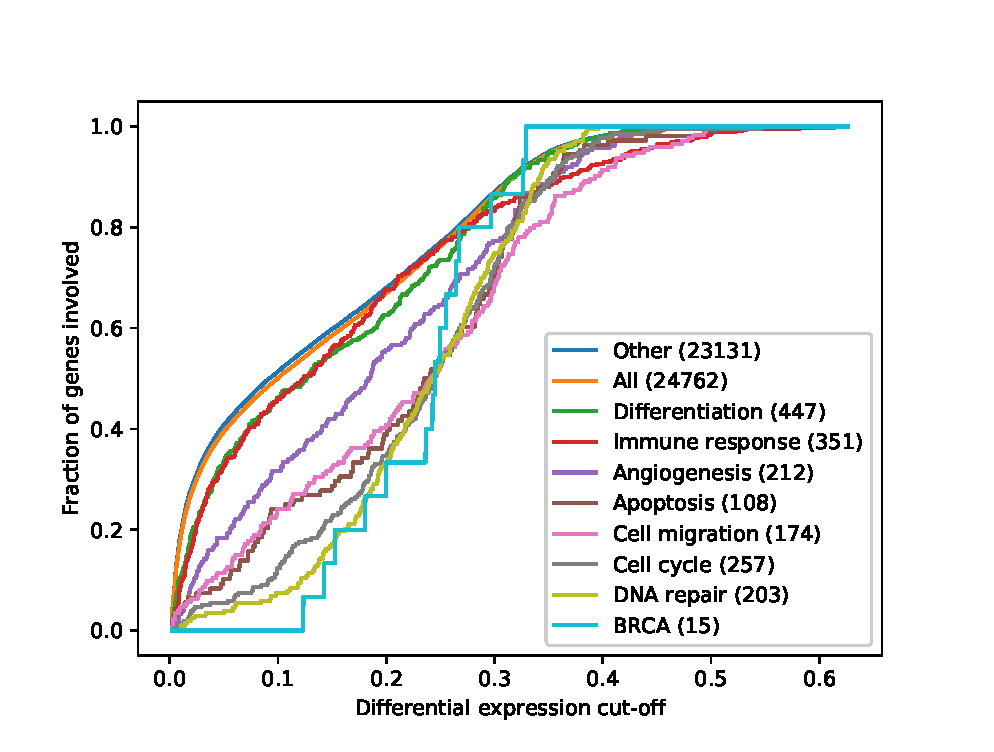
\includegraphics[width=0.9\textwidth]{3_proba_a/de2m_full}
	\end{center}
\end{frame}

%%%

\begin{frame}[t]{Differential expression (KS distance max/tumors)}{Most uniformly expressed among 400 most frequent GO terms}
	\begin{center}
		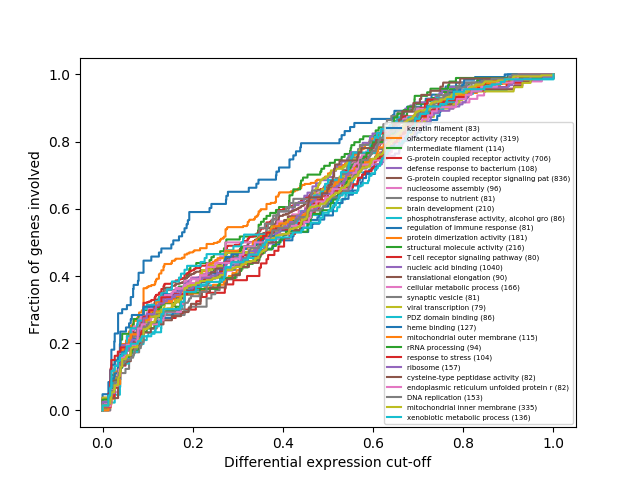
\includegraphics[width=0.9\textwidth]{3_proba_a/de2go_full}
	\end{center}
\end{frame}

%%%

\begin{frame}[t]{Sample-wise expression}{Overview}
	\begin{center}
		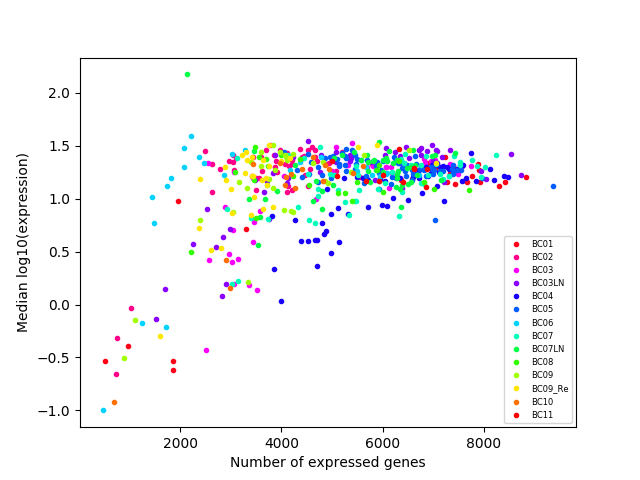
\includegraphics[width=0.9\textwidth]{2_stats_b/nnz-median}
	\end{center}
\end{frame}

%%%

\begin{frame}[t]{Sample-wise expression}{By batch (orange: median expression < 1)}
	\begin{center}
		\includegraphics<1> [width=0.8\textwidth]{2_stats_a/orig_BC01_XX}
		\includegraphics<2> [width=0.8\textwidth]{2_stats_a/orig_BC02_XX}
		\includegraphics<3> [width=0.8\textwidth]{2_stats_a/orig_BC03LN_XX}
		\includegraphics<4> [width=0.8\textwidth]{2_stats_a/orig_BC03_XX}
		\includegraphics<5> [width=0.8\textwidth]{2_stats_a/orig_BC04_XX}
		\includegraphics<6> [width=0.8\textwidth]{2_stats_a/orig_BC05_XX}
		\includegraphics<7> [width=0.8\textwidth]{2_stats_a/orig_BC06_XX}
		\includegraphics<8> [width=0.8\textwidth]{2_stats_a/orig_BC07LN_XX}
		\includegraphics<9> [width=0.8\textwidth]{2_stats_a/orig_BC07_XX}
		\includegraphics<10>[width=0.8\textwidth]{2_stats_a/orig_BC08_XX}
		\includegraphics<11>[width=0.8\textwidth]{2_stats_a/orig_BC09_Re_XX}
		\includegraphics<12>[width=0.8\textwidth]{2_stats_a/orig_BC09_XX}
		\includegraphics<13>[width=0.8\textwidth]{2_stats_a/orig_BC10_XX}
		\includegraphics<14>[width=0.8\textwidth]{2_stats_a/orig_BC11_XX}
	\end{center}
\end{frame}

%%%

\begin{frame}[t]{Random gene subset sampling, GO trace}{}
	{\only<1-3>{%
		\begin{center}
			\includegraphics<1>[width=0.7\textwidth]{6_low-high-end_a/go-freq_dims=10_filt=4}
			\includegraphics<2>[width=0.7\textwidth]{6_low-high-end_a/go-freq_dims=10_filt=16}
			\includegraphics<3>[width=0.7\textwidth]{6_low-high-end_a/go-freq_dims=10_filt=64}
		\end{center}
		
		\scriptsize 
		$10$ genes $\times$ $10^6$ random samples.
		Pick GO term if occurrence in sample $\geq$ expected.
		\\
		Top
		\only<1>{4}\only<2>{16}\only<3>{64}
		frequent GO terms, by median clustering index.
	}}%
	
	{\only<4-6>{%
		\begin{center}
			\includegraphics<4>[width=0.7\textwidth]{6_low-high-end_a/go-freq_dims=100_filt=4}
			\includegraphics<5>[width=0.7\textwidth]{6_low-high-end_a/go-freq_dims=100_filt=16}
			\includegraphics<6>[width=0.7\textwidth]{6_low-high-end_a/go-freq_dims=100_filt=64}
		\end{center}
		
		\scriptsize 
		$100$ genes $\times$ $10^6$ random samples.
		Pick GO term if occurrence in sample $\geq$ expected.
		\\
		Top
		\only<4>{4}\only<5>{16}\only<6>{64}
		frequent GO terms, by median clustering index.
	}}%
	
	{\only<7-9>{%
		\begin{center}
			\includegraphics<7>[width=0.7\textwidth]{6_low-high-end_a/go-freq_dims=1000_filt=4}
			\includegraphics<8>[width=0.7\textwidth]{6_low-high-end_a/go-freq_dims=1000_filt=16}
			\includegraphics<9>[width=0.7\textwidth]{6_low-high-end_a/go-freq_dims=1000_filt=64}
		\end{center}
		
		\scriptsize 
		$1000$ genes $\times$ $10^6$ random samples.
		Pick GO term if occurrence in sample $\geq$ expected.
		\\
		Top
		\only<7>{4}\only<8>{16}\only<9>{64}
		frequent GO terms, by median clustering index.
	}}%
\end{frame}

%%


%%%%%%%%%%%%%%%%%%%%%%%%%%%%%%%%%%%%%%%%%%%%%%%%%%%%%%%%%%%%%%%%%%%%%%%%%%%%%%%%%
%\section{Extra}
%%%%%%%%%%%%%%%%%%%%%%%%%%%%%%%%%%%%%%%%%%%%%%%%%%%%%%%%%%%%%%%%%%%%%%%%%%%%%%%%%
%
%
\newcounter{finalframe}
\setcounter{finalframe}{\value{framenumber}}
% Backup frames follow
%
%
%\begin{frame}
%	Appendix
%\end{frame}
%
%%
%
%\begin{frame}
%	%
%\end{frame}
%
%
% FINAL SLIDE
\setbeamercolor{background canvas}{bg=black}
\begin{frame}[plain,b]
	\hfill
	\tiny
	\color{gray}
	this slide is intentionally left blank
\end{frame}
\setbeamercolor{background canvas}{bg=white}


%%%%%%%%%%%%%%%%%%%%%%%%%%%%%%%%%%%%%%%%%%%%%%%%%%%%%%%%%%%%%%%%%%%%%%%%%%%%%%%%%
%\section{Bibliography}
%%%%%%%%%%%%%%%%%%%%%%%%%%%%%%%%%%%%%%%%%%%%%%%%%%%%%%%%%%%%%%%%%%%%%%%%%%%%%%%%%

% {
% \tiny
% \bibliography{../../../r/refs}
% }


%%%%%%%%%%%%%%%%%%%%%%%%%%%%%%%%%%%%%%%%%%%%%%%%%%%%%%%%%%%%%%%%%%%%%%%%%%%%%%%%
\setcounter{framenumber}{\value{finalframe}}
\end{document}
%%%%%%%%%%%%%%%%%%%%%%%%%%%%%%%%%%%%%%%%%%%%%%%%%%%%%%%%%%%%%%%%%%%%%%%%%%%%%%%%
%%%%%%%%%%%%%%%%%%%%%%%%%%%%%%%%%%%%%%%%%%%%%%%%%%%%%%%%%%%%%%%%%%%%%%%%%%%%%%%%

